\documentclass[border=8pt]{standalone}
\usepackage{tikz}
\usepackage{mathptmx}
\definecolor{navy}{RGB}{20,52,110}
\definecolor{accent}{RGB}{14,110,120}
\definecolor{orange}{RGB}{200,110,30}
\definecolor{gridg}{RGB}{170,170,170}
\begin{document}
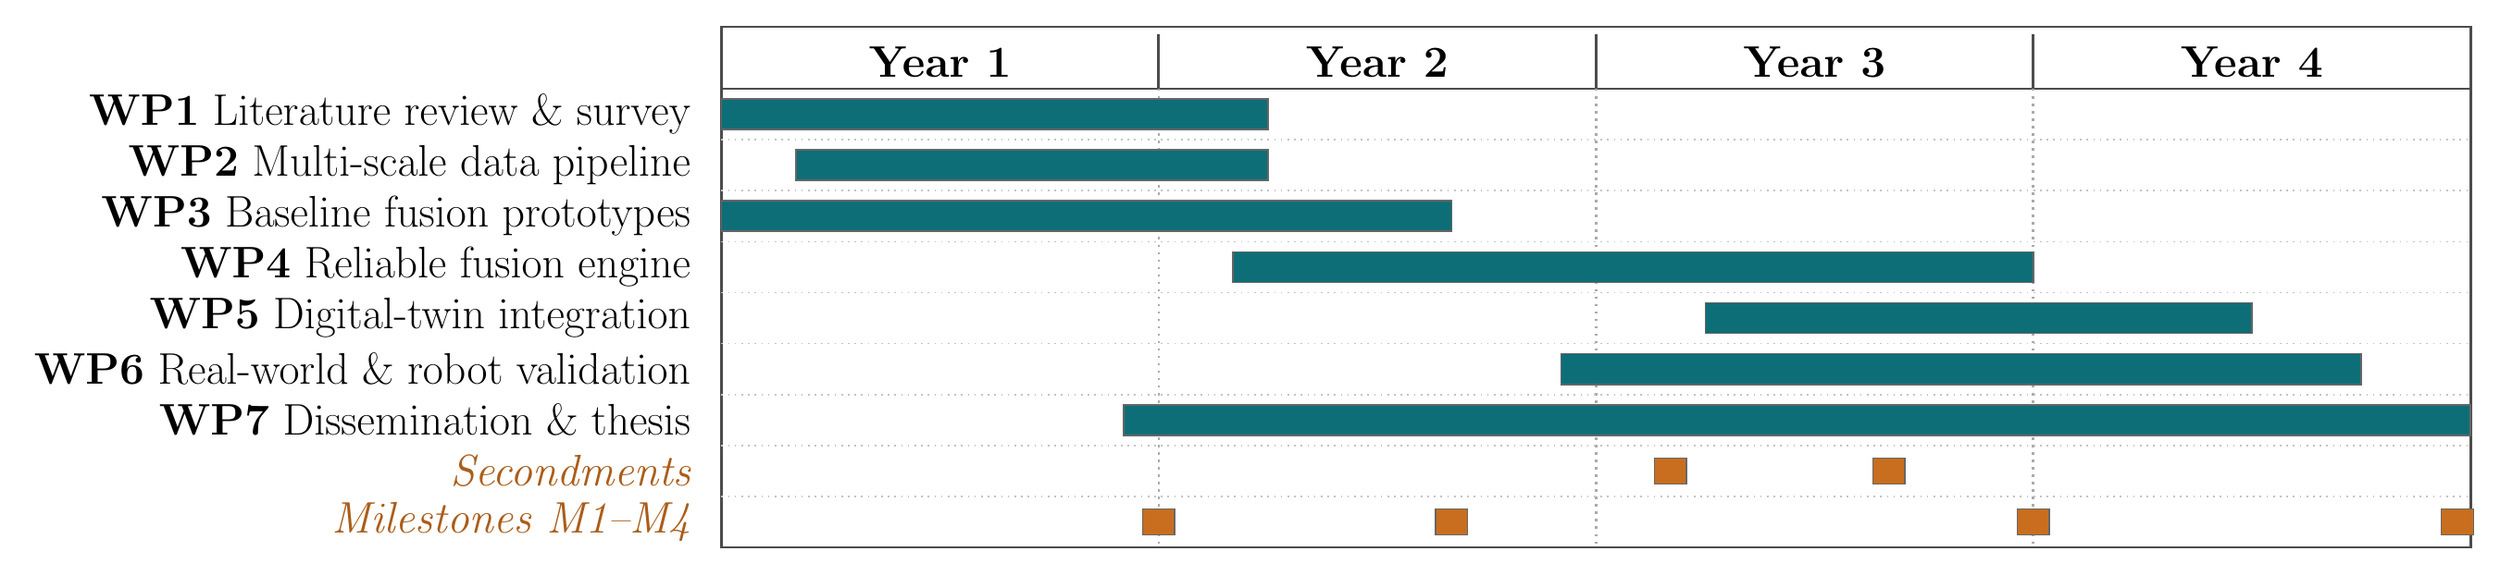
\begin{tikzpicture}[font=\sffamily]
% geometry: chart x in [0,24] (4 years x 6cm), rows 0.78cm tall
\def\rowh{0.70}
\def\barh{0.42}

% ---- year header band ----
\draw[line width=1pt, black!70] (0,0.85) rectangle (24,0);
\foreach \i/\yr in {0/Year 1, 1/Year 2, 2/Year 3, 3/Year 4}{
  \draw[line width=1pt, black!70] ({\i*6},0) -- ({\i*6},0.75);
  \node[font=\LARGE\bfseries] at ({\i*6+3},0.37) {\yr};
}

% ---- row grid + dotted year lines (9 rows) ----
\draw[line width=1pt, black!70] (0,0) rectangle (24,{-9*\rowh});
\foreach \i in {1,...,3}{ \draw[dotted, gridg, line width=0.9pt] ({\i*6},0) -- ({\i*6},{-9*\rowh}); }
\foreach \r in {1,...,8}{ \draw[dotted, gridg!70, line width=0.6pt] (0,{-\r*\rowh}) -- (24,{-\r*\rowh}); }

% ---- helper-free bars: {row}{start-year}{end-year} (years 0..4 -> x = yr*6)
% WP1 0 -> 1.25
\fill[accent, draw=black!60, line width=0.6pt] (0,{-0*\rowh-(\rowh-\barh)/2-\barh}) rectangle ({1.25*6},{-0*\rowh-(\rowh-\barh)/2});
% WP2 0.17 -> 1.25
\fill[accent, draw=black!60, line width=0.6pt] ({0.17*6},{-1*\rowh-(\rowh-\barh)/2-\barh}) rectangle ({1.25*6},{-1*\rowh-(\rowh-\barh)/2});
% WP3 0 -> 1.67
\fill[accent, draw=black!60, line width=0.6pt] (0,{-2*\rowh-(\rowh-\barh)/2-\barh}) rectangle ({1.67*6},{-2*\rowh-(\rowh-\barh)/2});
% WP4 1.17 -> 3.0
\fill[accent, draw=black!60, line width=0.6pt] ({1.17*6},{-3*\rowh-(\rowh-\barh)/2-\barh}) rectangle ({3.0*6},{-3*\rowh-(\rowh-\barh)/2});
% WP5 2.25 -> 3.5
\fill[accent, draw=black!60, line width=0.6pt] ({2.25*6},{-4*\rowh-(\rowh-\barh)/2-\barh}) rectangle ({3.5*6},{-4*\rowh-(\rowh-\barh)/2});
% WP6 1.92 -> 3.75
\fill[accent, draw=black!60, line width=0.6pt] ({1.92*6},{-5*\rowh-(\rowh-\barh)/2-\barh}) rectangle ({3.75*6},{-5*\rowh-(\rowh-\barh)/2});
% WP7 0.92 -> 4.0
\fill[accent, draw=black!60, line width=0.6pt] ({0.92*6},{-6*\rowh-(\rowh-\barh)/2-\barh}) rectangle ({4.0*6},{-6*\rowh-(\rowh-\barh)/2});

% ---- secondments (orange squares, row 7) ----
\foreach \x in {2.17, 2.67}{
  \fill[orange, draw=black!60, line width=0.5pt]
    ({\x*6-0.22},{-7*\rowh-\rowh/2-0.18}) rectangle ({\x*6+0.22},{-7*\rowh-\rowh/2+0.18});
}
% ---- milestones (orange squares, row 8) ----
\foreach \x in {1.0, 1.67, 3.0, 3.97}{
  \fill[orange, draw=black!60, line width=0.5pt]
    ({\x*6-0.22},{-8*\rowh-\rowh/2-0.18}) rectangle ({\x*6+0.22},{-8*\rowh-\rowh/2+0.18});
}

% ---- left labels (large) ----
\node[anchor=east, font=\LARGE] at (-0.3,{-0*\rowh-\rowh/2}) {\textbf{WP1} Literature review \& survey};
\node[anchor=east, font=\LARGE] at (-0.3,{-1*\rowh-\rowh/2}) {\textbf{WP2} Multi-scale data pipeline};
\node[anchor=east, font=\LARGE] at (-0.3,{-2*\rowh-\rowh/2}) {\textbf{WP3} Baseline fusion prototypes};
\node[anchor=east, font=\LARGE] at (-0.3,{-3*\rowh-\rowh/2}) {\textbf{WP4} Reliable fusion engine};
\node[anchor=east, font=\LARGE] at (-0.3,{-4*\rowh-\rowh/2}) {\textbf{WP5} Digital-twin integration};
\node[anchor=east, font=\LARGE] at (-0.3,{-5*\rowh-\rowh/2}) {\textbf{WP6} Real-world \& robot validation};
\node[anchor=east, font=\LARGE] at (-0.3,{-6*\rowh-\rowh/2}) {\textbf{WP7} Dissemination \& thesis};
\node[anchor=east, font=\LARGE\itshape, color=orange!85!black] at (-0.3,{-7*\rowh-\rowh/2}) {Secondments};
\node[anchor=east, font=\LARGE\itshape, color=orange!85!black] at (-0.3,{-8*\rowh-\rowh/2}) {Milestones M1--M4};
\end{tikzpicture}
\end{document}
